 \documentclass[xcolor=dvipsnames,table]{beamer}

\usepackage{latexsym}
\usepackage[utf8]{inputenc}
\usepackage[brazil]{babel}
\usepackage{amssymb}
\usepackage{amsmath}
\usepackage{stmaryrd}
\usepackage{fancybox}
\usepackage{datetime}
\usepackage[T1]{fontenc}
\usepackage{graphicx}
\usepackage{graphics}
\usepackage{url}
\usepackage{algorithmic}
\usepackage{algorithm}
\usepackage{acronym}
\usepackage{array}

\newtheorem{definicao}{Definio}
\newcommand{\tab}{\hspace*{2em}}

\mode<presentation>
{
  \definecolor{colortexto}{RGB}{0,0,0}
 
  \setbeamertemplate{background canvas}[vertical shading][ bottom=white!10,top=white!10]
  \setbeamercolor{normal text}{fg=colortexto} 

  \usetheme{Warsaw}
}

\title{Apresentação da Disciplina}  

\author{
  Esdras Lins Bispo Jr. \\ \url{bispojr@ufj.edu.br}
  } 
 \institute{
  Lógica para Ciência da Computação \\Bacharelado em Ciência da Computação}
\date{\textbf{19 de março de 2026} }

\logo{
\includegraphics[width=1.5cm]{images/ufjJataiLogo.png}}

\begin{document}

	\begin{frame}
		\titlepage
	\end{frame}

	\AtBeginSection{
		\begin{frame}{Sumário}%[allowframebreaks]{Sumário}
    		\tableofcontents[currentsection]
    		%\tableofcontents[currentsection, hideothersubsections]
		\end{frame}
	}

	\begin{frame}{Plano de Aula}
		\tableofcontents
		%\tableofcontents[hideallsubsections]
	\end{frame}
	
	\section{Sobre a Disciplina}
	\subsection{Professor}
	\begin{frame}{Professor}
		\begin{columns}
			\column{.4\textwidth}  		
			\begin{center}
				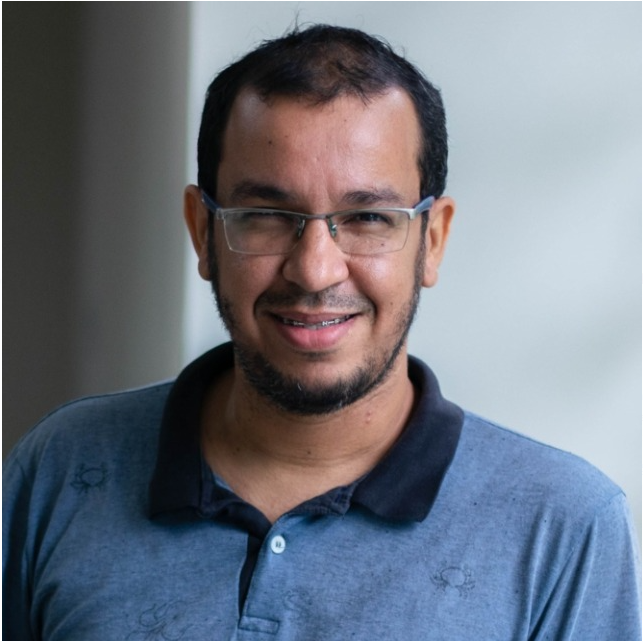
\includegraphics[height=.5\textheight]{images/eu-quadrado.png}
			\end{center}
			\column{.6 \textwidth}  		
			\begin{block}{Quem?}
				\begin{center}
					{\bf Esdras Lins Bispo Junior} \\ Recife, Pernambuco.
				\end{center}
			\end{block}
			\begin{block}{Formação}
				\begin{center}
					{\normalsize Sistemas de Informação (Grad.)\\
                    Inteligência Artificial (Mest.)\\
                    Educação em Computação (Dout.)}
				\end{center}
			\end{block}	
			\begin{block}{Linha de Pesquisa}
				Equidade na Educação em Computação
			\end{block}
		\end{columns}
	\end{frame}
	
	\subsection{Informações Importantes}
	\begin{frame}{Informações Importantes}
		\begin{block}{Professor}
			\begin{itemize}
				\item Esdras Lins Bispo Jr.
				\item \url{bispojr@ufj.edu.br}
				\item Sala 18, 1º Andar (Bloco dos Professores, próx. CA2)
			\end{itemize}
		\end{block}
	\end{frame}	
	
	\begin{frame}{Informações Importantes}
		\begin{block}{Disciplina}
			\begin{itemize}
				\item Lógica para Ciência da Computação (ICE 0239)
				\item 15h30-17h10 (Terça, [CA1, Sala 01])\\
				 09h30-11h10 (Quinta, [CA1, Sala 01])
				\item Dúvidas: 11h10  (Quinta)\\
				{\color{red}[é necessário confirmação comigo]}
				%\item Google Clasroom: Código - {\color{blue} \bf sufpjv5}
				\item Repositório: ???
			\end{itemize}
		\end{block}
	\end{frame}	
	
	\begin{frame}{Informações Importantes}
		\begin{block}{Metodologia}
			\begin{itemize}
				\item Instrução pelos Colegas (IpC);
				\item Exercícios em Sala;
				\item Listas de Exercícios;
				\item Testes.
			\end{itemize}
		\end{block}
	\end{frame}

	\begin{frame}{Plickers}
	\begin{center}
		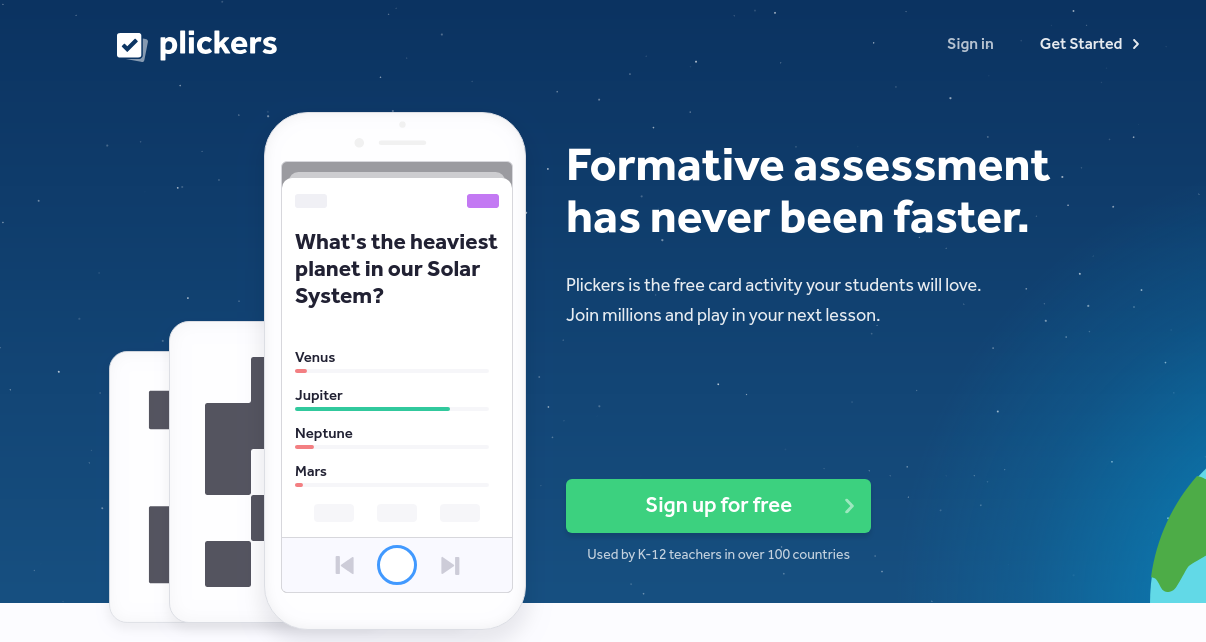
\includegraphics[width=\textwidth]{images/plickers}
	\end{center}
\end{frame}
	
	\begin{frame}{Metodologia IpC}
		\begin{center}
			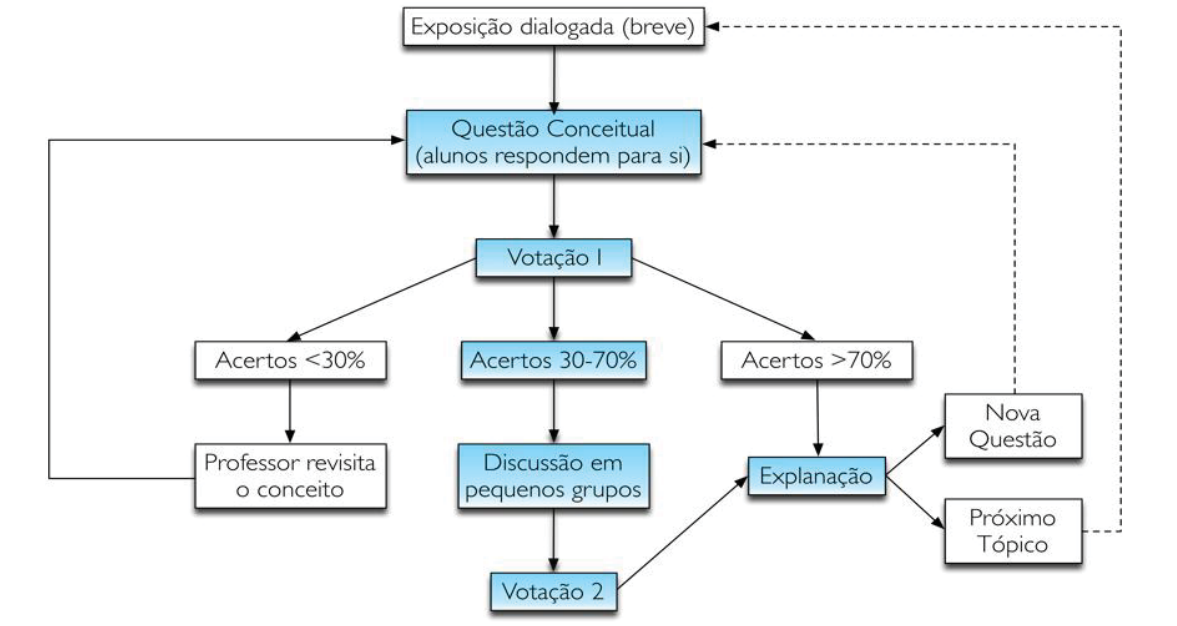
\includegraphics[height=.7\textheight]{images/fluxo-ipc}
		\end{center}
	\end{frame}

		\begin{frame}{Rotina Acadêmica}
			\begin{block}{Estudo Prévio}
				Antes de cada aula, haverá um material disponível para estudo prévio.
			\end{block}	\pause
			\begin{block}{Questões Conceituais IpC (QC)}
				Toda aula haverá questões conceituais abordadas em sala.
			\end{block}
		\end{frame}
\section{Avaliação}
\subsection{Perspectivas}
\begin{frame}{Perspectivas sobre Avaliação}
    \begin{block}{Gestor x Formador}
        \begin{itemize}
            \item Gestor $\Rightarrow$ Excelência;
            \item Formador $\Rightarrow$ Aprendizagem.
        \end{itemize}
    \end{block} \pause
    \begin{exampleblock}{Qual é a principal função do professor?}
        \begin{itemize}
            \item Promover a excelência ou a aprendizagem?
            \item Parceiro ou Juiz?
        \end{itemize}
    \end{exampleblock}
\end{frame}

\begin{frame}{Avaliação Formativa}
    \begin{block}{Foco da Avaliação (PPC)}
        ``A avaliação deverá enfatizar o {\bf processo formativo} em detrimento da modalidade classificatória, desvinculando-se do âmbito da promoção/retenção para o âmbito da observação, do diagnóstico, acompanhados de registros sistemáticos de situações formais e informais'' (BCC, 2022, p. 67).
    \end{block} 
    \begin{exampleblock}{Projeto Pedagógico do Curso (PPC)}
        PPC | Bacharelado em Ciência da Computação (BCC):
        \url{https://computacao.jatai.ufg.br/p/3492-documentos}
    \end{exampleblock} \pause
    \begin{block}{Pressupostos Básicos}
        \begin{itemize}
            \item (i) O professor quer ensinar, e (ii) O aluno quer aprender
        \end{itemize}
    \end{block}
\end{frame}

\begin{frame}{Avaliação Formativa}
	\begin{center}
		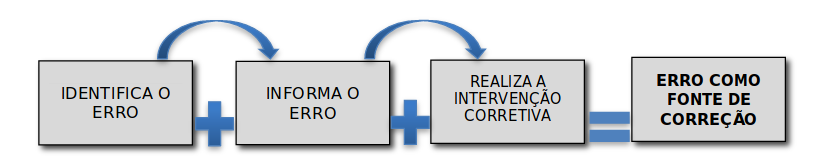
\includegraphics[width=\textwidth]{images/fluxo-correcao} \pause
		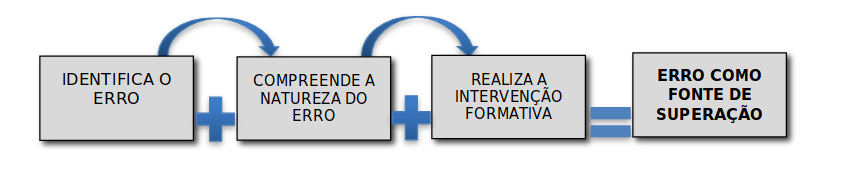
\includegraphics[width=\textwidth]{images/fluxo-superacao}
	\end{center}
\end{frame}

\begin{frame}{Avaliação Formativa}
    \begin{block}{Foco da Avaliação (PPC)}
        ``A avaliação deve servir, em primeiro lugar, para {\bf reorientar o aprendiz} no desenvolvimento das aprendizagens e o professor, no replanejamento das atividades. Não pode ser, pois, meramente classificatória, mas uma ferramenta construtiva, que promove melhorias e inovações, com vistas ao {\bf aperfeiçoamento da aprendizagem}. Aos alunos, após discussão sobre o processo, os instrumentos e os resultados da avaliação, devem ser propiciados meios que lhes permitam sanar dificuldades evidenciadas e realizar as aprendizagens em níveis crescentes de desenvolvimento.'' (BCC, 2022, p. 67).
    \end{block}
\end{frame}

\subsection{Instrumentos}

\begin{frame}{Instrumentos de Avaliação}
    \begin{block}{Critérios de Aprovação}
    	\begin{itemize}
    		\item Estar presente em 75\% dos nossos encontros;
    		\item Compromisso com a própria aprendizagem ($\cong$ 2h);
    		\item Realizar todas as nossas avaliações.
    	\end{itemize}
    \end{block} \pause
    \begin{exampleblock}{Nota Final}
    	Média Final = 6,0 + Autoavaliação Dialogada [0,0 a 4,0]
    \end{exampleblock}
\end{frame}

\begin{frame}{Instrumentos de Avaliação}
    \begin{block}{Motivos para Sinalizar o Descomprometimento}
        \begin{itemize}
            \item Por você (potencial humano)
            \item Pela turma (garantia do direito)
            \item Pela sociedade (prestação do uso do recurso)
        \end{itemize}
    \end{block}
\end{frame}

\begin{frame}{Instrumentos de Avaliação}
    \begin{block}{Critérios de Reprovação}
        \begin{itemize}
            \item Ausência em 25\% dos nossos encontros ou mais;
            \item Descomprometimento com a própria aprendizagem após as avaliações.
        \end{itemize}
    \end{block} \pause
    \begin{alertblock}{Nota Final}
        \begin{itemize}
            \item Média Final = 4,0.
        \end{itemize}
        
    \end{alertblock}
\end{frame}

\begin{frame}{Instrumentos de Avaliação}

    \begin{block}{Testes}
        \begin{itemize}
            \item T$_1$, T$_2$, T$_3$, e T$_4$
        \end{itemize}
    \end{block} \pause

    \begin{block}{Substitutivas}
		Cada teste terá ao menos um momento de caráter substitutivo: \pause 
		\begin{itemize}
			\item o ST$_1$ (referente ao T$_1$), 
			\item o ST$_2$ (referente ao T$_2$),
            \item o ST$_3$ (referente ao T$_3$), e 
			\item o ST$_4$ (referente ao T$_4$).
		\end{itemize} \pause
		
		\begin{itemize}
			
		\end{itemize}
	\end{block}
	
\end{frame}

\section{Conteúdo da Disciplina}
	
	\begin{frame}{Informações Importantes}
		\begin{block}{Conteúdo do Curso}
			\begin{enumerate}
				\item Lógica Proposicional;
				\item Relações em Lógica Proposicional;
				\item Demonstrações;
				\item Lógica de Predicados.
			\end{enumerate}
		\end{block}
	\end{frame}

    \begin{frame}{Próxima Aula}
    \begin{block}{Leitura Prévia}
        \begin{itemize}
            \item {\bf \color{blue} [L1]} ALENCAR FILHO, E. {\bf Iniciação à Lógica Matemática}, 1a Edição, Editora Nobel, 2002. \\{\color{blue} \bf Código Bib.: [510.6 ALE/ini]}.
        \end{itemize}
    \end{block}
    \begin{block}{Páginas}
        \begin{itemize}
        \item {\bf Aula 03 (24/03)}: Capítulo 1 (pp. 11-15) {\bf \color{blue} [L1]} 
        \end{itemize}
    \end{block}
\end{frame}
	
	\begin{frame}
		\titlepage
	\end{frame}
	
\end{document}